\documentclass{article}

\usepackage{amsmath, amsfonts, microtype, xcolor, tikz, graphicx, hyperref, amsthm}
\usepackage[ruled, linesnumbered]{algorithm2e}
\usepackage[]{neurips_2019}
\newtheorem{theorem}{Theorem}


\title{Measuring causal influence with\\ back-to-back regression: the linear case - supplementary material}

\begin{document}

\appendix

\maketitle

\section{Additional Figures}

\begin{figure}[h]
  \centering
  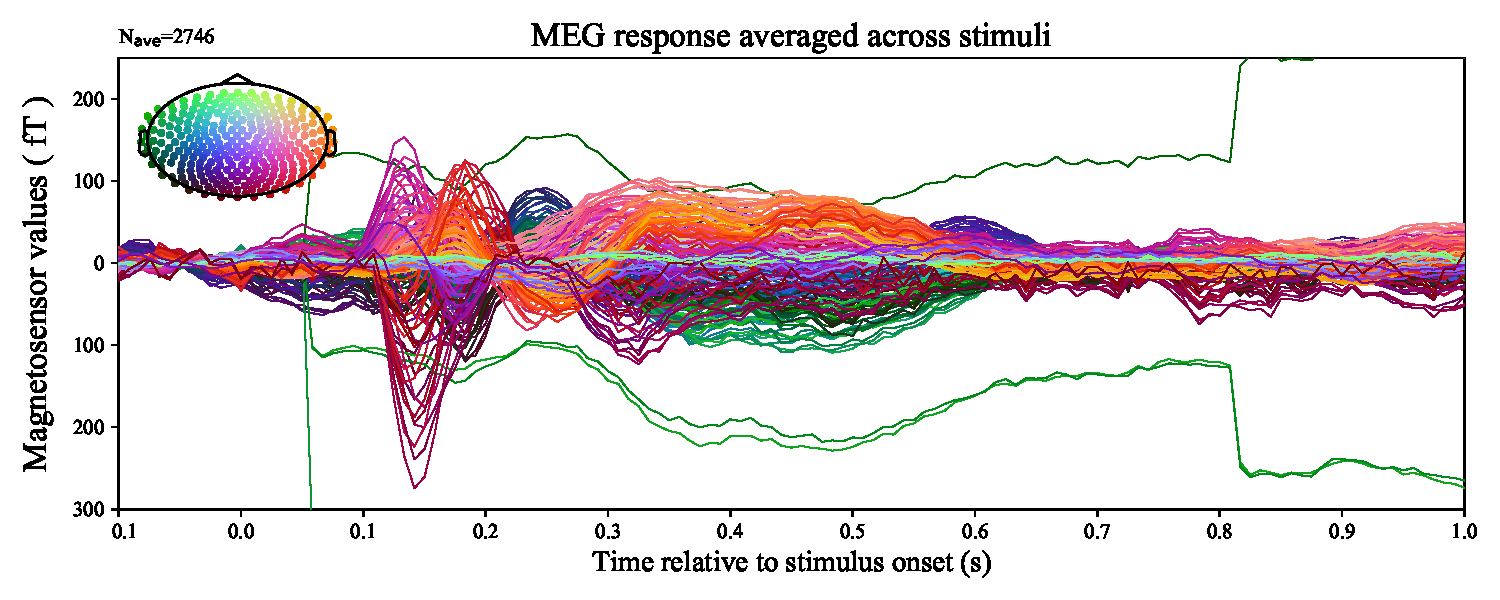
\includegraphics[width=\textwidth, trim=0cm 0cm 0cm 0cm, clip=True]{figures/meg_sensors.pdf}
  \caption{Magnetosensor response (femtoteslas fT) averaged across words for the first subject. The color coding corresponds to the positions of the sensors on the head as shown on the top-left diagram. The diverging curves correspond to artifacts in the MEG data.}
  \label{fig:megavg}
\end{figure}


\begin{figure}[h]
  \centering
  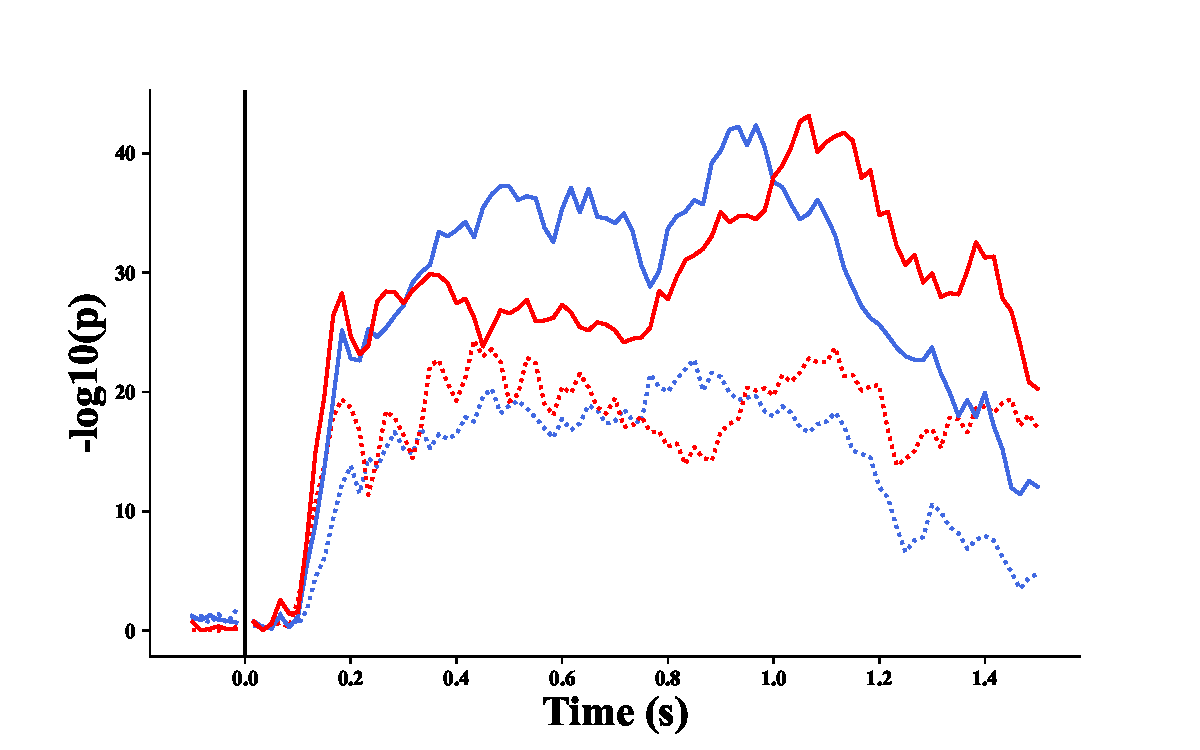
\includegraphics[width=\textwidth, trim=0cm 0cm 0cm 0cm]{figures/pvalues.pdf}
  \caption{We apply a statistical t-test to measure if coefficients were significantly different from baseline value (at word onset, $t=0$ms).
  We compute the negative logarithm of the p-value (\textit{higher is better}: nonzero effects are more easily detected). We plot the average across features, over time. Red: word length, blue: word frequency.
  Full line: B2B, dashed line: Forward regression. We see that our method more easily detects the influence of causes of MEG response.}
\end{figure}


\begin{figure}[h]
  \centering
  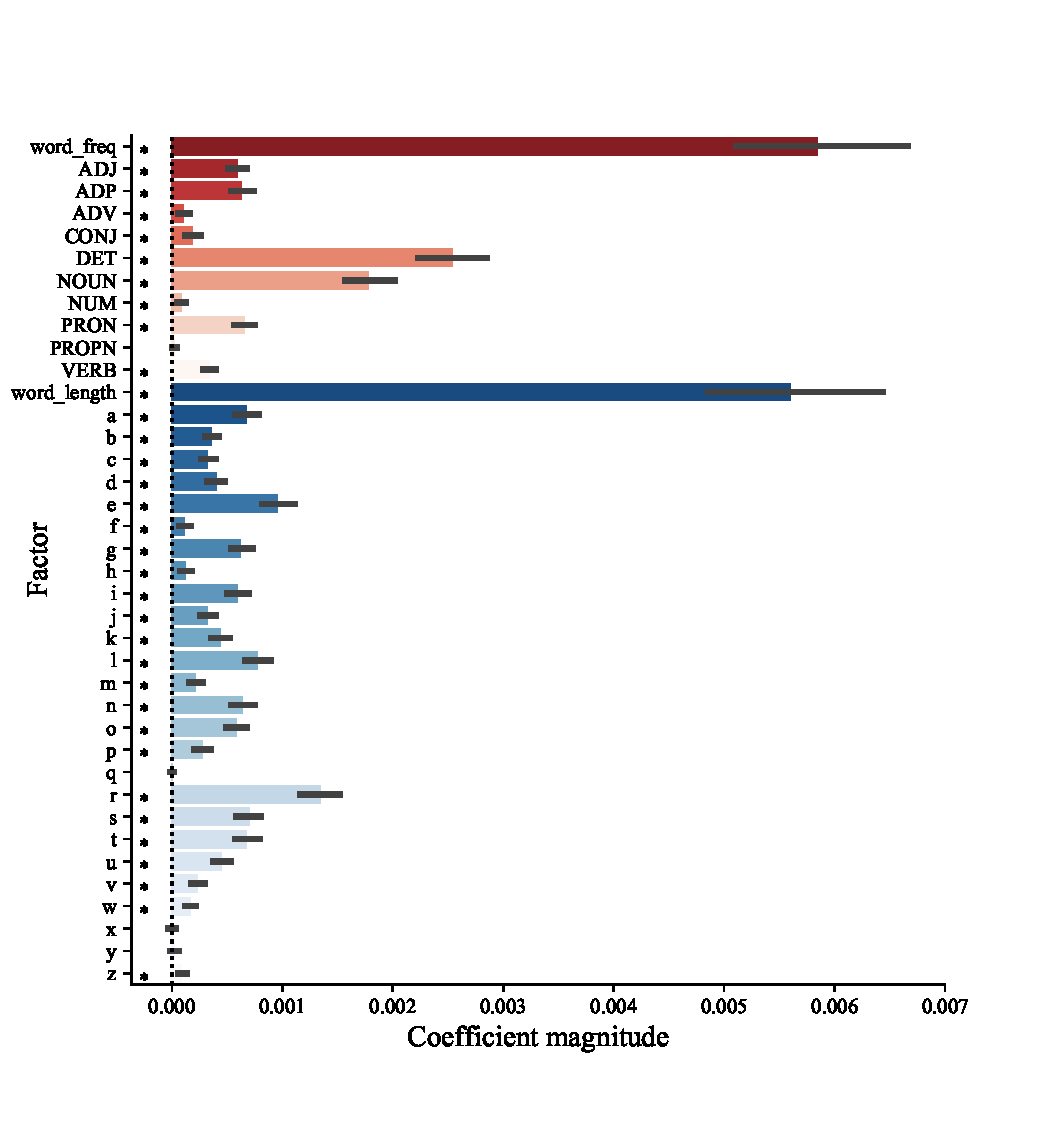
\includegraphics[width=\textwidth, trim=0cm 0cm 0cm 0cm]{figures/pvalues_vertical.pdf}
  \caption{We show the average value and the standard deviation across subjects of the coefficients obtained with our method during the trials. the $\star$  symbol corresponds to statistically significant (t-test) nonzero values.}
  \label{fig:ridgebaselineresult}
\end{figure}

\clearpage
\newpage

\section{Additional Theorems}

\setcounter{theorem}{1}
 \begin{theorem}[B2B consistency, general case]

     Consider the B2B model from Equation $Y = (XE + N)F$, with centered, full-rank noise $N$.
     %
     If $F$ and $X$ are full-rank on $\text{Img}(E)$, then, the solution of B2B, $\hat H$, will minimise
     %
     $\min_H  \left \| X - XH\right\| ^2  + \left \| NH\right \| ^2$and satisfy $E\hat H = \hat H$
\end{theorem}
\begin{proof}

 Let $\hat G$ and $\hat H$ be the solutions of the first and second regressions of B2B, we have
 \begin{align*}
    \hat G = \arg \min_G \mathbb{E}[\left \| YG - X \right \|^2] &=   \arg \min_G \mathbb{E}[\left \| X - (XE + N)FG \right\|^2]\\
                                                        &{}= \arg \min_G \mathbb{E}[\left \| X - XEFG\right\| ^2]  + \mathbb{E}[\left \| NFG\right \| ^2]\\
                                                        &{}= \arg \min_G \left \| X - XEFG\right\| ^2  + \left \| NFG\right \| ^2,
     \label{eq:doublenorm}
\end{align*}
\begin{align*}
    \hat H = \arg \min_H \mathbb{E}[\| XH - Y \hat{G} \|^2] &=\arg  \min_H \mathbb{E}[\| XH - (XE + N)F \hat G \|^2] \\
    &=\arg \min_H \mathbb{E}[\| X(H - EF \hat G) \| ^2] + \mathbb{E}[\| NF\hat G \| ^2]\\
    &= \arg \min_H \mathbb{E}[\| X(H - EF \hat G) \| ^2]\\
    &= EF \hat G.
\end{align*}
%
First, we show that $EF\hat G = F\hat G$.
%
Let $Z=F^\dagger EF\hat G$. We have $FZ = FF^\dagger EF  \hat G= EF\hat G$.
Then, $FF^\dagger E =E$ since $F$ is full rank on $\text{Img}(E)$.
%
Since $E$ is a contraction, we have $ \| NEF\hat G\|^2 \leq \| NF\hat G \|^2$. Therefore, 
 $$\left \| X - XEFZ\right \| ^2  + \left \| NFZ\right \| ^2 = \| X - XEF\hat G \| ^2  + \| NEF\hat G \| ^2 \leq \| X - XEF\hat G \| ^2  + \| NF\hat G \| ^2.$$

But as $\hat G =  \arg \min_G \left \| X - XEFG\right\| ^2  + \left \| NFG\right \| ^2$, the above inequality is an equality, $Z=\hat G$ and $EF\hat G = F\Hat G$.

Therefore, $\left \| X - XEFG\right \| ^2  + \left \| NFG\right \| ^2 = \left \| X - XEFG\right \| ^2  + \left \| NEFG\right \| ^2 = \left \| X - XH\right \| ^2  + \left \| NH\right \| ^2$ is minimised by $\hat G$ and $\hat H$. 

Finally, $E\hat H = E EF\hat G = EF\hat G = \hat H$. This completes the proof.
\end{proof}

So, $\hat H = \arg \min_H  \left \| X - XEH\right\| ^2  + \left \| NEH\right \| ^2 = (E X^\top XE +EN^\top NE) ^\dagger EXX^\top$.

Assuming, without loss of generality, that the active features are the $k$ first, we have 

$X^\top X = \left(\begin{array}{lccl}\Sigma_{X1} & \Sigma_{X2} \\ \Sigma_{X2} & \Sigma_{X3}\end{array}\right)$, $N^\top N = \left(\begin{array}{lccl}\Sigma_{N1} & \Sigma_{N2} \\ \Sigma_{N2} & \Sigma_{N3}\end{array}\right)$ and 

$\hat H = \left(\begin{array}{cc}(\Sigma_{X1}+\Sigma_{N1})^{-1}\Sigma_{X1} & (\Sigma_{X1}+\Sigma_{N1})^{-1}\Sigma_{X2} \\0 & 0\end{array}\right)$

    $\text{Diag}_k (\hat H) = \text{Diag}((\Sigma_{X1}+\Sigma_{N1})^{-1}\Sigma_{X1}) = \text{Diag}((I+\Sigma_{X1}^{-1}\Sigma_{N1})^{-1})$

In the absence of noise, we have $\text{Diag}(\hat H) = \text{Diag}(E)$. Else the k first diagonal elements of $\hat H$ are all positive, and bounded by $\frac{\sigma_{X_k}}{\sigma_{X_k} +\sigma_{N_1}}$ and $\frac{\sigma_{X_1}}{\sigma_{X_1} +\sigma_{N_k}}$, where  $\sigma_{X_1}$, $\sigma_{X_k}$, $\sigma_{N_1}$ and $\sigma_{N_k}$ denote the largest and smallest eigenvalues of $\Sigma_{X1}$ and $\Sigma_{N1}$.

The average value of the coefficients of $\text{Diag}(\hat H)$ is the trace of $\hat H$ divided by k. On average, since $X$ and $N$ are not correlated, $\Sigma_{X1}^{-1}\Sigma_{N1}$ should have a low condition numbers, and $\frac{Var(X)}{Var(X)+Var(N)}$ provide a good estimate of $\frac{1}{k}Tr(\hat H)$.

\end{document}
